\subsection{Controller block}\label{chapter_CONTROLLER_BLOCK}
The figure below shows the content of the light blue 'Control' block in figure \ref{fig:MATLAB Overview}.
\begin{figure}[H]
	\centering
		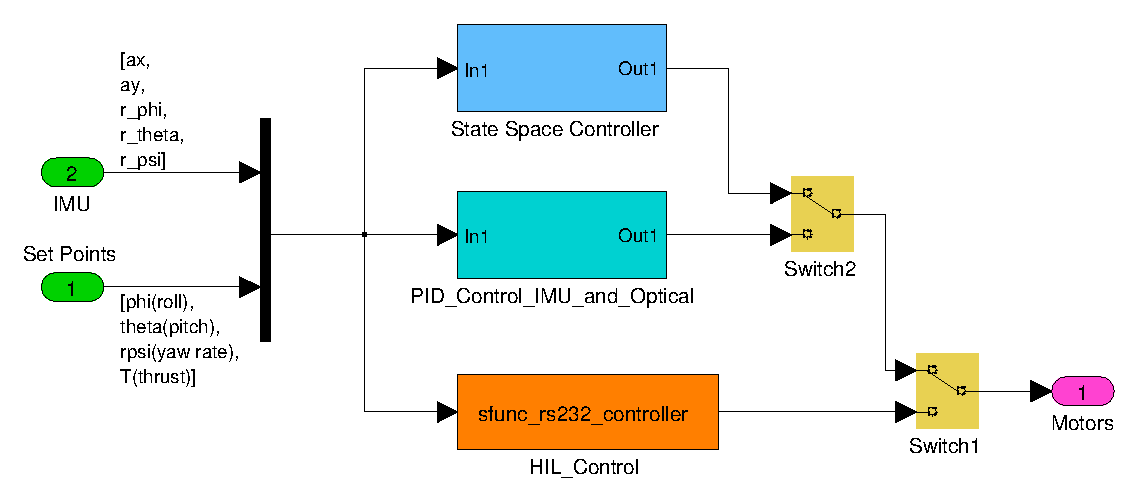
\includegraphics[width=1.0\textwidth]{03_Grafiken/MATLAB_Controller.pdf}
	\caption{Controller block}
	\label{fig:Controller block}
\end{figure}
The controller block has two inputs, 'Set Points' and sensor values ('IMU'). The black bar combines them to one vector with the elements:
\begin{enumerate*}
	\item \textit{ax} (acceleration in direction of x of bodyframe; IMU)
	\item \textit{ay} (acceleration in direction of y of bodyframe; IMU)
	\item \textit{rphi} (rate of phi; IMU)
	\item \textit{rtheta} (rate of theta; IMU)
	\item \textit{rpsi} (rate of psi; IMU)
	\item \textit{phi} (Set point of phi)
	\item \textit{theta} (Set point of theta)
	\item \textit{rpsi} (Set point or rate of psi)
	\item \textit{thrust} (Set point of thrust)
\end{enumerate*}
This vector is the input of three blocks. The topmost, light blue block is the new state space controller, implemented in this project. The second block, pictured in cyan, is the, already existing, PID-controller. The lowermost, orange block is the block, that is used to test the quadrocopter hardware in the loop (HIL).
The two switches on the right side define, which controller is enabled or rather whose actuating variables are connected to the process. The output of each controller block are the 'pseudo forces', every propeller has to provide.